\documentclass[../DefinizioneDiProdotto.tex]{subfiles}
\begin{document}
		\section{Specifica delle componenti}
			\subsection{SWEDesigner}
				I package contenuti al suo interno sono:
				\begin{itemize}
					\item SWEDesigner::Client;
					\item SWEDesigner::Server.
				\end{itemize}
				Questo package non contiene delle classi.
			\subsection{SWEDesigner::Client}
				% IMMAGINE ARCHITETTURA CLIENT GENERALE
				\begin{figure}[H]\label{fig:ClientSubsystem}
					\centering
					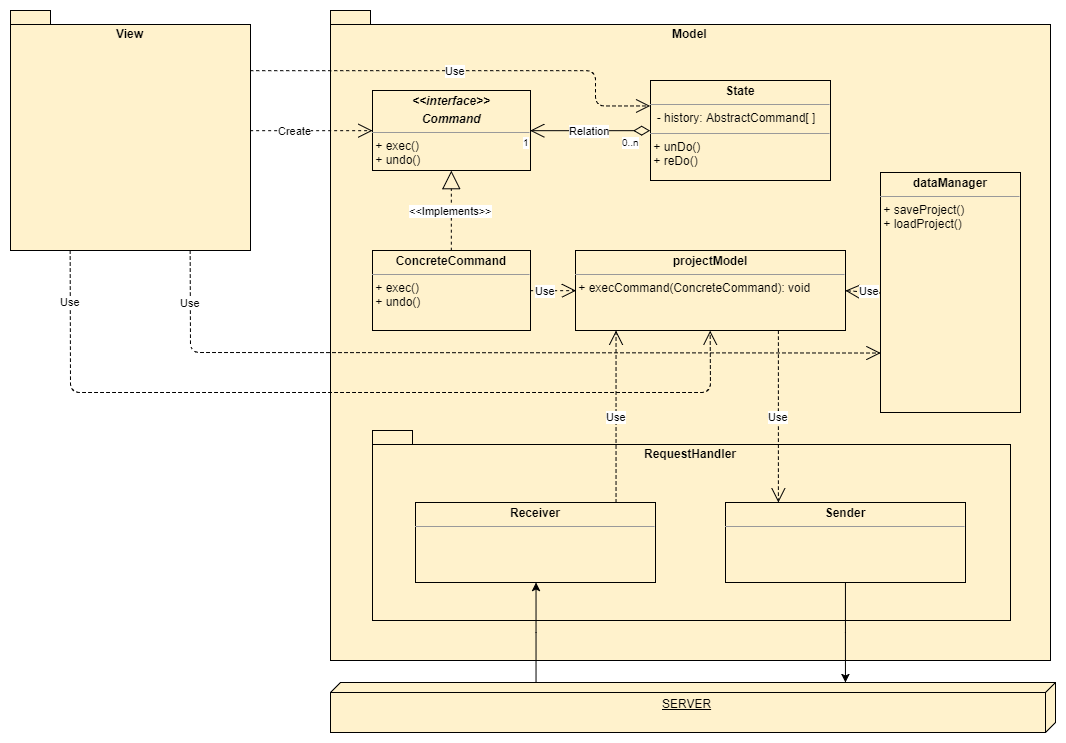
\includegraphics[scale=0.46]{Immagini/DiagrammaArchitettura/ClientSubsystem.png}
					\caption{Architettura del client}
				\end{figure}
				I package contenuti al suo interno sono:
				\begin{itemize}
					\item SWEDesigner::Client::Model;
					\item SWEDesigner::Client::View.
				\end{itemize}
				Questo package non contiene delle classi.
			\subsection{SWEDesigner::Client::Model}
				\hypertarget{SWEDesigner::Client::Model}
				I package contenuti al suo interno sono:
				\begin{itemize}
					\item SWEDesigner::Client::Model::RequestHandler.
				\end{itemize}
				Le classi contenute al suo interno verranno elencate qui di seguito.
				\subsubsection{SWEDesigner::Client::Model::Command}
				È l'interfaccia che rappresenta un generico comando impartito dai moduli View ai Model.\\
					FAN-IN:
					\begin{itemize}
						\item ConcreteCommand: implementa l'interfaccia Command per la rappresentazione concreta dei singoli comandi impartiti dai moduli View ai Model;
						\item View: il componente del programma che si occupa di gestire l'interfaccia grafica;
						\item State: gestisce la cronologia delle operazioni svolte permettendo le operazioni di unDo e reDo.
					\end{itemize}
					Non ci sono dipendenze OUT.

				\subsubsection{SWEDesigner::Client::Model::ConcreteCommand}
				Implementa l'interfaccia Command per la rappresentazione concreta dei singoli comandi impartiti dai moduli View ai Model.\\
					Non ci sono dipendenze IN.\\
					FAN-OUT:
					\begin{itemize}
						\item Command: è l'interfaccia che rappresenta un generico comando impartito dai moduli View ai Model;
						\item projectModel: si occupa di gestire la parte logica dell'editor.
					\end{itemize}

				\subsubsection{SWEDesigner::Client::Model::State}
				\hypertarget{SWEDesigner::Client::Model::State}
				Gestisce la cronologia delle operazioni svolte permettendo le operazioni di unDo e reDo.\\
					FAN-IN:
					\begin{itemize}
						\item View: il componente del programma che si occupa di gestire l'interfaccia grafica.
					\end{itemize}
					FAN-OUT:
					\begin{itemize}
						\item Command: è l'interfaccia che rappresenta un generico comando impartito dai moduli View ai Model.
					\end{itemize}

				\subsubsection{SWEDesigner::Client::Model::dataManager}
				\hypertarget{SWEDesigner::Client::Model::dataManager}
				Si occupa della persistenza dei dati, in particolare del salvataggio su file system locale del progetto già esistente.\\
					FAN-IN:
					\begin{itemize}
						\item View: il componente del programma che si occupa di gestire l'interfaccia grafica.
					\end{itemize}
					FAN-OUT:
					\begin{itemize}
						\item projectModel: si occupa di gestire la parte logica dell'editor;
						\item project: si occupa di gestire gli elementi contenuti nel diagramma.
					\end{itemize}

				\subsubsection{SWEDesigner::Client::Model::projectModel}
					% IMMAGINE ARCHITETTURA MAINMODEL
					\begin{figure}[H]\label{fig:Model}
						\centering
						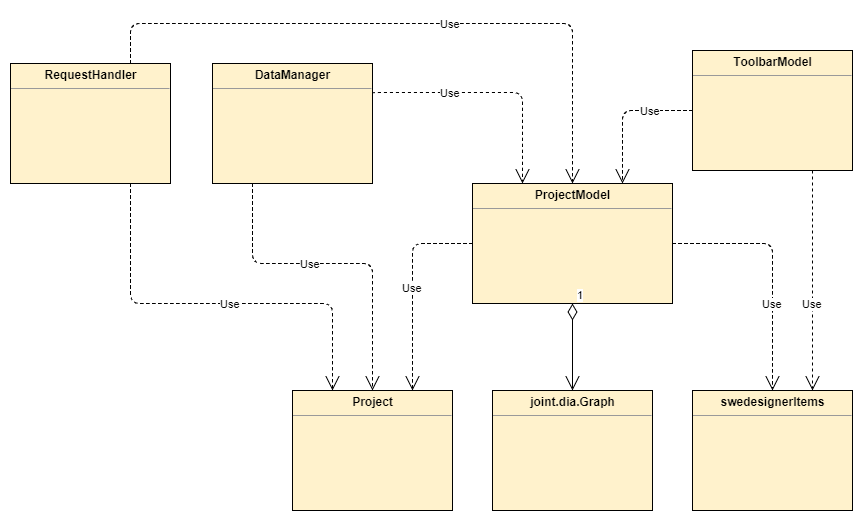
\includegraphics[scale=0.46]{Immagini/DiagrammaArchitettura/MainModel.png}
						\caption{Architettura di Model}
					\end{figure}

				È il componente del programma che si occupa di gestire la parte logica dell’editor.\\
					FAN-IN:
					\begin{itemize}
						\item ConcreteCommand: rappresenta i comandi inviati dalle View ed eseguiti poi da Model;
						\item dataManager: si occupa della persistenza dei dati, in particolare del salvataggio su file system locale del progetto e del caricamento di un progetto già esistente;
						\item View: invoca il metodo execCommand;
						\item Client::RequestHandler::Receiver: si occupa di gestire i dati ricevuti dal server.
					\end{itemize}
					FAN-OUT:
					\begin{itemize}
						\item Client::RequestHandler::Sender: si occupa di gestire le comunicazioni in uscita verso il server.
					\end{itemize}

				\subsubsection{SWEDesigner::Client::Model::toolbarModel}
				È il componente del programma che si occupa di gestire la parte logica della toolbar.\\
					FAN-IN:\\
					Non ci sono dipendenze IN. \\
					FAN-OUT:
					\begin{itemize}
						\item projectModel: si occupa di gestire la parte logica dell'editor;
						\item swedesignerItems: definisce il comportamento degli oggetti contenuti nel diagramma.
					\end{itemize}

				\subsubsection{SWEDesigner::Client::Model::project}
				si occupa di gestire gli elementi contenuti nel diagramma.\\
					FAN-IN:
					\begin{itemize}
						\item projectModel: si occupa di gestire la parte logica dell'editor;
						\item dataManager: Si occupa della persistenza dei dati, in particolare del salvataggio su file system locale del progetto già esistente;
						\item requestHandler: Si occupa di gestire le comunicazioni con il server.
					\end{itemize}
					FAN-OUT:\\
					Non ci sono dipendenze OUT. \\
				
			\subsection{SWEDesigner::Client::Model::RequestHandler}
				\hypertarget{SWEDesigner::Client::Model::RequestHandler}
				Questo package non contiene dei sottopackage.\\
				Le classi contenute al suo interno verranno elencate qui di seguito.
				\subsubsection{SWEDesigner::Client::Model::RequestHandler::Sender}
				Si occupa di gestire le comunicazioni in uscita verso il server.\\
					FAN-IN:
					\begin{itemize}
						\item View: ne invoca i metodi.
					\end{itemize}
					FAN-OUT:
					\begin{itemize}
						\item projectModel: si occupa di gestire la parte logica dell'editor;
						\item project: si occupa di gestire gli elementi contenuti nel diagramma;
						\item Server::RequestHandler::Receiver: si occupa di gestire le comunicazioni in entrata dal Client.
					\end{itemize}

				\subsubsection{SWEDesigner::Client::Model::RequestHandler::Receiver}
				Si occupa di gestire le comunicazioni in entrata dal server.\\
					FAN-IN:
					\begin{itemize}
						\item Server::RequestHandler::Sender: si occupa di gestire le comunicazioni in uscita verso il Client.
					\end{itemize}
					FAN-OUT:
					\begin{itemize}
						\item projectModel: si occupa di gestire la parte logica dell'editor;
						\item project: si occupa di gestire gli elementi contenuti nel diagramma.
					\end{itemize}

			\subsection{SWEDesigner::Client::View}
				\hypertarget{SWEDesigner::Client::View}{}
				È il componente del programma che si occupa di gestire l'interfaccia grafica. Nella particolare declinazione MVC adottata da Backbone.js, si occupa anche di gestire gli input dell'utente.
				% IMMAGINE ARCHITETTURA VIEW
					\begin{figure}[H]\label{fig:View}
						\centering
						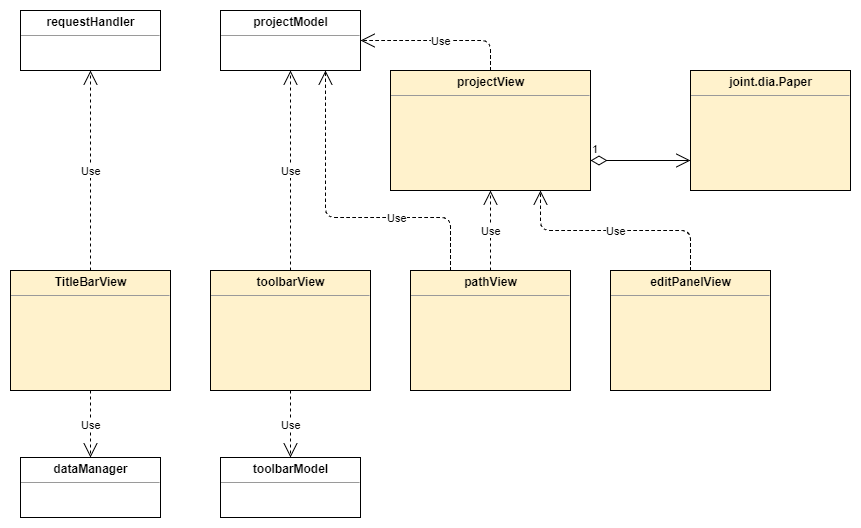
\includegraphics[scale=0.44]{Immagini/DiagrammaArchitettura/View.png}
						\caption{Architettura di View}
					\end{figure}
				Questo package non contiene dei sottopackage.
				Le classi contenute al suo interno verranno elencate qui di seguito.

				\subsubsection{SWEDesigner::Client::View::projectView}
					\hypertarget{SWEDesigner::Client::View::projectView}{}
						\begin{itemize}
						\item \textbf{Tipo}: \emph{Class};
						\item \textbf{Descrizione}: Questa classe gestisce il diagramma disegnato e le interazioni dell'utente con esso;
						\item \textbf{Padre}: \hyperlink{SWEDesigner::Client::View}{\emph{SWEDesigner::Client::View}};
						\item \textbf{Attributi}:
						\begin{itemize}
							\item \emph{model} \\
							Istanza di \hyperlink{SWEDesigner::Model::projectModel}{\emph{projectModel}} del programma;
							\item \emph{paper} \\
							Oggetto joint.dia.Paper della libreria esterna JointJS;
						\end{itemize}
						\item \textbf{Metodi}:
						\begin{itemize}
							\item \emph{resetSelectedCell(): void} \\
							Pone this.paper.selectedCell a null e genera l'evento "changed-selected-cell";
							\item \emph{mouseMoveFunction(event: JavaScriptEvent): void} \\
							Provoca la traslazione del paper nella direzione del trascinamento del mouse; \\
							Parametri:
							\begin{itemize}
								\item \emph{event: JavaScriptEvent}: Evento;
							\end{itemize}
							\item \emph{blankPointerDown(elem: cellView, event: JavaScriptEvent, x: double, y: double): void} \\
							Salva le correnti coordinate al click del mouse nello spazio vuoto del paper; \\
							Parametri:
							\begin{itemize}
								\item \emph{elem: cellView}: Elemento cellView;
								\item \emph{event: JavaScriptEvent}: Evento;
								\item \emph{x: double}: Coordinata dell'asse delle ascisse;
								\item \emph{y: double}: Coordinata dell'asse delle ordinate;
							\end{itemize}
							\item \emph{blankPointerUp(elem: cellView, event: JavaScriptEvent, x: double, y: double): void} \\
							Elimina le coordinate iniziali al click del mouse nello spazio vuoto del paper; \\
							Parametri:
							\begin{itemize}
								\item \emph{elem: cellView}: Elemento cellView;
								\item \emph{event: JavaScriptEvent}: Evento;
								\item \emph{x: double}: Coordinata dell'asse delle ascisse;
								\item \emph{y: double}: Coordinata dell'asse delle ordinate;
							\end{itemize}
							\item \emph{onMouseWheel(elem: cellView, event: JavaScriptEvent): void} \\
							Trasla verticalmente il paper effettuando uno zoom in avanti o indietro a seconda della rotazione della ruota del mouse; \\
							Parametri:
							\begin{itemize}
								\item \emph{elem: cellView}: Elemento cellView;
								\item \emph{event: JavaScriptEvent}: Evento;
							\end{itemize}
							\item \emph{render(): void} \\
							Provoca il render della projectVIew;
							\item \emph{addCell(elem: cellView, event: JavaScriptEvent, x: double, y: double): void} \\
							Aggiunge un nuovo elemento al graph chiamando il relativo metodo di \hyperlink{SWEDesigner::Model::projectModel}{\emph{projectModel}}; \\
							Parametri:
							\begin{itemize}
								\item \emph{elem: cellView}: Elemento cellView;
								\item \emph{event: JavaScriptEvent}: Evento;
								\item \emph{x: double}: Coordinata dell'asse delle ascisse;
								\item \emph{y: double}: Coordinata dell'asse delle ordinate;
							\end{itemize}
							\item \emph{deleteCell(event: JavaScriptEvent): void} \\
							Elimina un elemento dal graph chiamando il relativo metodo di ProjectModel;\\
							Parametri:
							\begin{itemize}
								\item \emph{event: JavaScriptEvent}: Evento;
							\end{itemize}
							\item \emph{unembedCell(event: JavaScriptEvent): void} \\
							Rimuove l'innestamento della cella selezionata;\\
							Parametri:
							\begin{itemize}
								\item \emph{event: JavaScriptEvent}: Evento;
							\end{itemize}
							\item \emph{pointerDownFunction(prView: \hyperlink{SWEDesigner::Client::View::projectView}{\emph{projectView}}, elem: cellView, event: JavaScriptEvent, x: double, y: double): void} \\
							Gestice l'evento generato dal click (non rilasciato) del mouse nel paper. Se viene cliccato un elemento, genera a sua volta l'evento "changed-selected-cell" gestito da \hyperlink{SWEDesigner::Client::View::EditPanelView}{\emph{EditPanelView}};\\
							Parametri:
							\begin{itemize}
								\item \emph{prView: \hyperlink{SWEDesigner::Client::View::projectView}{\emph{projectView}}}: Istanza di projectView;
								\item \emph{elem: cellView}: Elemento cellView;
								\item \emph{event: JavaScriptEvent}: Evento;
								\item \emph{x: double}: Coordinata dell'asse delle ascisse;
								\item \emph{y: double}: Coordinata dell'asse delle ordinate;
							\end{itemize}
							\item \emph{pointerUpFunction(prView: \hyperlink{SWEDesigner::Client::View::projectView}{\emph{projectView}}, elem: cellView, event: JavaScriptEvent, x: double, y: double): void} \\
							Gestice l'evento generato dal click (al rilascio) del mouse nel paper (rimozione di un elemento, nesting di un elemento in un'altro, collegamento di una relazione tra elementi);\\
							Parametri:
							\begin{itemize}
								\item \emph{prView: \hyperlink{SWEDesigner::Client::View::projectView}{\emph{projectView}}}: Istanza di projectView;
								\item \emph{elem: cellView}: Elemento cellView;
								\item \emph{event: JavaScriptEvent}: Evento;
								\item \emph{x: double}: Coordinata dell'asse delle ascisse;
								\item \emph{y: double}: Coordinata dell'asse delle ordinate;
							\end{itemize}
							\item \emph{switchIn(id: string): void} \\
							Gestisce lo switch in profondità (dall'elemento selezionato il cui id è parametro in input) invocando il relativo metodo di \hyperlink{SWEDesigner::Model::projectModel}{\emph{projectModel}};\\
							Parametri:
							\begin{itemize}
								\item \emph{id: string}: Identificativo dell'elemento;
							\end{itemize}
							\item \emph{switchOut(diagramType: string): void} \\
							Gestisce lo switch verso un diagramma (il cui tipo è parametro in input) antistante da quello corrente invocando il relativo metodo di \hyperlink{SWEDesigner::Model::projectModel}{\emph{projectModel}}.\\
							Parametri:
							\begin{itemize}
								\item \emph{diagramType: string}: Tipo di diagramma di destinazione;
							\end{itemize}
							\item \emph{deleteOperationAt(ind: int): void} \\
							Gestisce l'eliminazione di un diagramma delle bubble invocando il relativo metodo di \hyperlink{SWEDesigner::Model::projectModel}{\emph{projectModel}}.\\
							Parametri:
							\begin{itemize}
								\item \emph{ind: int}: Indice dell'array di operazioni del diagramma delle bubble da eliminare;
							\end{itemize}
						\end{itemize}
						FAN-IN:
						\begin{itemize}
							\item pathView: gestisce l'interfaccia grafica della barra di indirizzo;
							\item editPanelView: gestisce l'interfaccia grafica del pannello di editing.
						\end{itemize}
						FAN-OUT:
						\begin{itemize}
							\item projectModel: si occupa di gestire la parte logica dell'editor;
							\item Paper: gestisce l'interfaccia grafica dell'area dei diagrammi.
						\end{itemize}
					\end{itemize}
					

				\subsubsection{SWEDesigner::Client::View::titlebarView}
				È il componente del programma che fa la funzione di view per la barra del titolo, dove saranno collocati il menu dell’applicazione e gli shortcut.\\
					FAN-IN:\\
					Non ci sono dipendenze IN.\\
					FAN-OUT:
					\begin{itemize}
						\item requestHandler: gestisce la comunicazione con il server;
						\item dataManager: gestisce la persistenza dei dati su file system.
					\end{itemize}

				\subsubsection{SWEDesigner::Client::View::toolbarView}
				È il componente del programma che fa la funzione di view per la toolbar dove saranno collocati gli strumenti per editare i diagrammi.\\
					FAN-IN:\\
					Non ci sono dipendenze IN.\\
					FAN-OUT:
					\begin{itemize}
						\item projectModel: si occupa di gestire la parte logica dell'editor;
						\item toolbarModel: si occupa di gestire la parte logica della toolbar.
					\end{itemize}

				\subsubsection{SWEDesigner::Client::View::pathView}
				È il componente del programma che fa la funzione di view per il cosiddetto breadcrumb dove viene inserita la posizione corrente.\\
					FAN-IN:
					Non ci sono dipendenze IN. \\
					FAN-OUT:
					\begin{itemize}
						\item projectModel: si occupa di gestire la parte logica dell'editor;
						\item projectView: si occupa di gestire la parte grafica del model.
					\end{itemize}
				
				\subsubsection{SWEDesigner::Client::View::EditPanelView}
				È il componente del programma che fa la funzione di view per le informazioni editabili degli elementi che fanno parte dei diversi diagrammi.\\
					FAN-IN:\\
					Non ci sono dipendenze IN. \\
					FAN-OUT:
					\begin{itemize}
						\item projectView: si occupa di gestire la parte grafica del model.
					\end{itemize}
			
			\subsection{SWEDesigner::Server}
				% IMMAGINE ARCHITETTURA SERVER GENERALE
				\begin{figure}[H]\label{fig:ServerSubsystem}
					\centering
					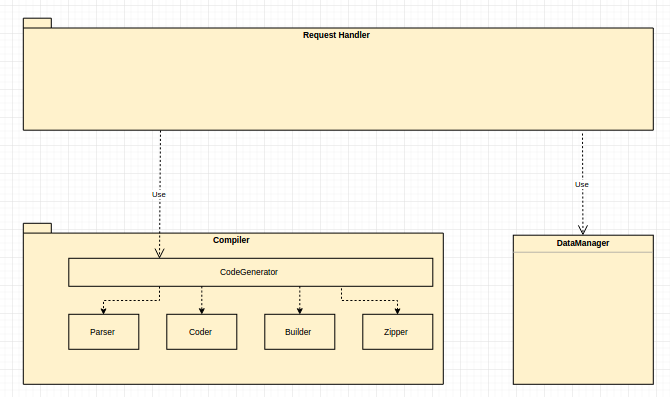
\includegraphics[scale=0.4]{Immagini/DiagrammaArchitettura/ServerSubsystem.png}
					\caption{Architettura del server}
				\end{figure}
				I package contenuti al suo interno sono:
				\begin{itemize}
					\item SWEDesigner::Server::CodeGenerator;
					\item SWEDesigner::Server::DAORequestHandler;
					\item SWEDesigner::Server::RequestHandler.
				\end{itemize}
				Questo package non contiene delle classi.

			\subsection{SWEDesigner::Server::CodeGenerator}
				I package contenuti al suo interno sono:
				\begin{itemize}
					\item SWEDesigner::Server::CodeGenerator::Builder;
					\item SWEDesigner::Server::CodeGenerator::Coder;
					\item SWEDesigner::Server::CodeGenerator::Parser;
					\item SWEDesigner::Server::CodeGenerator::Zipper.
				\end{itemize}
				Le classi contenute al suo interno verranno elencate qui di seguito.

				\subsubsection{SWEDesigner::Server::CodeGenerator::CodeGenerator}
				\hypertarget{SWEDesigner::Server::CodeGenerator::CodeGenerator}
				E' il componente che rende disponibile la funzionalità per cui, dato un file valido in formato JSON, restituisce un pacchetto in formato .zip contenente i file del codice sorgente che costituiscono il programma rappresentato dal file in input. I file prodotti sono strutturati in packages, come indicato nel file JSON in input.\\
					FAN-IN:
					\begin{itemize}
						\item Server::RequestHandler::Receiver: si occupa di gestire le comunicazioni in entrata dal client.
					\end{itemize}
					FAN-OUT:
					\begin{itemize}
						\item Server::RequestHandler::Sender: si occupa di gestire le comunicazioni in uscita verso il client;
						\item Parser: si occupa di creare un oggetto che contiene le informazioni ricevute in input;
						\item Coder: si occupa della traduzione in codice dell'oggetto ottenuto dal Parser;
						\item Builder: si occupa di organizzare in maniera organica il codice generato dal Coder;
						\item Zipper: si occupa di creare un archivio .zip contenente in codici sorgente precedentemente creati.
					\end{itemize}

			\subsection{SWEDesigner::Server::CodeGenerator::Builder}
				Questo package non contiene dei sottopackage.\\
				Le classi contenute al suo interno verranno elencate qui di seguito.
				\subsubsection{SWEDesigner::Server::CodeGenerator::Builder::Builder}
				È il componente che rende disponibile la funzionalità, dato un file JSON in input che rappresenti un programma, di ottenere un oggetto contenitore del codice sorgente corrispondente al contenuto del file di input. Tale codice è suddiviso e strutturato come indicato nel file di input.\\
					FAN-IN:
					\begin{itemize}
						\item Zipper: si occupa di creare un archivio .zip contenente in codici sorgente precedentemente creati.
					\end{itemize}
					FAN-OUT:
					\begin{itemize}
						\item Coder: componente che funge da interfaccia alle operazioni di codifica di una stringa permettendo quindi di trasformare le informazioni del file in formato JSON in codice sorgente.
					\end{itemize}

			\subsection{SWEDesigner::Server::CodeGenerator::Coder}
				% IMMAGINE ARCHITETTURA CODER
				\begin{figure}[H]\label{fig:Coder}
					\centering
					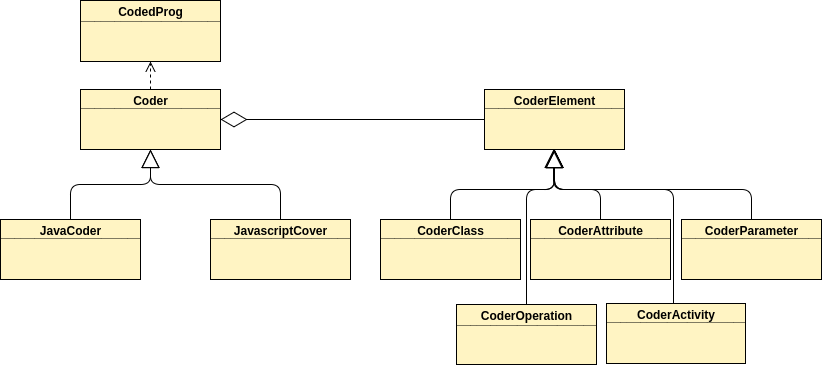
\includegraphics[scale=0.46]{Immagini/DiagrammaArchitettura/Coder.png}
					\caption{Architettura di Coder}
				\end{figure}

				Questo package non contiene dei sottopackage.\\
				Le classi contenute al suo interno verranno elencate qui di seguito.
				\subsubsection{SWEDesigner::Server::CodeGenerator::Coder::Coder}
				Componente che funge da interfaccia alle operazioni di codifica di una stringa, in formato JSON che rappresenta un programma valido; tali operazioni permettono di ottenere un oggetto contenente il codice sorgente, in Java o Javascript, corrispondente alla stringa in input.\\
					FAN-IN:
					\begin{itemize}
						\item JavaCoder: si occupa di trasformare un oggetto JSON ricevuto in input in un oggetto contenente il codice sorgente scritto in java;
						\item JavaScriptCoder: si occupa di trasformare un oggetto JSON ricevuto in input in un oggetto contenente il codice sorgente scritto in javascript.
					\end{itemize}
					FAN-OUT:
					\begin{itemize}
						\item CodedProg: componente che contiene il codice prodotto dal Coder;
						\item CoderElement: componente astratto che offre la funzionalità che permette di associare ad ogni stringa contenuta nel file JSON il corrispondente codice sorgente.
					\end{itemize}

				\subsubsection{SWEDesigner::Server::CodeGenerator::Coder::JavaCoder}
				È il componente che rende disponibile la funzionalità, dato un oggetto in input che rappresenta un file JSON parsificato, di ottenere un oggetto contenente il codice sorgente, in linguaggio Java, corrispondente all'oggetto in input.\\
					Non ci sono dipendenze IN.\\
					FAN-OUT:
					\begin{itemize}
						\item Coder: componente che funge da interfaccia alle operazioni di codifica di una stringa permettendo quindi di trasformare le informazioni del file in formato JSON in codice sorgente.
					\end{itemize}

				\subsubsection{SWEDesigner::Server::CodeGenerator::Coder::JavascriptCoder}
				È il componente che rende disponibile la funzionalità, dato un oggetto in input che rappresenta un file JSON parsificato, di ottenere un oggetto contenente il codice sorgente, in linguaggio Javascript, corrispondente all'oggetto in input.\\
					Non ci sono dipendenze IN.\\
					FAN-OUT:
					\begin{itemize}
						\item Coder: componente che funge da interfaccia alle operazioni di codifica di una stringa permettendo quindi di trasformare le informazioni del file in formato JSON in codice sorgente.
					\end{itemize}

				\subsubsection{SWEDesigner::Server::CodeGenerator::Coder::CoderClass}
				È il componente che mette a disposizione la funzionalità, data una stringa in input in formato JSON che rappresenta una classe valida, di ottenere il corrispondente codice sorgente di tale classe.\\
					Non ci sono dipendenze IN.\\
					FAN-OUT:
					\begin{itemize}
						\item CoderElement: componente astratto che offre la funzionalità che permette di associare ad ogni stringa contenuta nel file JSON il corrispondente codice sorgente.
					\end{itemize}

				\subsubsection{SWEDesigner::Server::CodeGenerator::Coder::CoderOperation}
				È il componente che mette a disposizione la funzionalità, data una stringa in input in formato JSON che rappresenta un'operazione valida, di ottenere il corrispondente codice sorgente di tale operazione.\\
					Non ci sono dipendenze IN.\\
					FAN-OUT:
					\begin{itemize}
						\item CoderElement: componente astratto che offre la funzionalità che permette di associare ad ogni stringa contenuta nel file JSON il corrispondente codice sorgente.
					\end{itemize}

				\subsubsection{SWEDesigner::Server::CodeGenerator::Coder::CoderParameter}
				È il componente che mette a disposizione la funzionalità, data una stringa in input in formato JSON che rappresenta un parametro di una lista valido, di ottenere il corrispondente codice sorgente di tale parametro. È possibile scegliere fra la codifica in Java o Javascript.\\
					Non ci sono dipendenze IN.\\
					FAN-OUT:
					\begin{itemize}
						\item CoderElement: componente astratto che offre la funzionalità che permette di associare ad ogni stringa contenuta nel file JSON il corrispondente codice sorgente.
					\end{itemize}

				\subsubsection{SWEDesigner::Server::CodeGenerator::Coder::CoderAttribute}
				È il componente che mette a disposizione la funzionalità, data una stringa in input in formato JSON che rappresenta un attributo valido, di ottenere il corrispondente codice sorgente di tale attributo. È possibile scegliere fra la codifica in Java o Javascript.\\
				Non ci sono dipendenze IN.\\
					FAN-OUT:
					\begin{itemize}
						\item CoderElement: componente astratto che offre la funzionalità che permette di associare ad ogni stringa contenuta nel file JSON il corrispondente codice sorgente.
					\end{itemize}

				\subsubsection{SWEDesigner::Server::CodeGenerator::Coder::CoderActivity}
				È il componente che mette a disposizione la funzionalità, data una stringa in input in formato JSON che rappresenta un diagramma delle attività valido, di ottenere il corrispondente codice sorgente di tale attività. È possibile scegliere fra la codifica in Java o Javascript.\\
					Non ci sono dipendenze IN.\\
					FAN-OUT:
					\begin{itemize}
						\item CoderElement: componente astratto che offre la funzionalità che permette di associare ad ogni stringa contenuta nel file JSON il corrispondente codice sorgente;
						\item DAO: si occupa di gestire il database delle bubble.
					\end{itemize}

				\subsubsection{SWEDesigner::Server::CodeGenerator::Coder::CodedProg}
				È il componente che contiene il codice sorgente prodotto dal Coder.\\
					FAN-IN:
					\begin{itemize}
						\item Coder: componente che funge da interfaccia alle operazioni di codifica di una stringa permettendo quindi di trasformare le informazioni del file in formato JSON in codice sorgente.
					\end{itemize}
					Non ci sono dipendenze OUT.
				
				\subsubsection{SWEDesigner::Server::CodeGenerator::Coder::CoderElement}
				Componente astratta che offre la funzionalità di ottenere, data una stringa in input in formato JSON che rappresenta un elemento di classe valido, il corrispondente codice sorgente, in Java o Javascript.\\
					FAN-IN:
					\begin{itemize}
						\item Coder: componente che funge da interfaccia alle operazioni di codifica di una stringa permettendo quindi di trasformare le informazioni del file in formato JSON in codice sorgente;
						\item CoderClass: componente che permette data una stringa in input in formato JSON che rappresenta un diagramma delle classi valido, di ottenere il corrispondente codice sorgente di tale classe;
						\item CoderOperations: componente che permette data una stringa in input in formato JSON che rappresenta un'operazione valida, di ottenere il corrispondente codice sorgente di tale operazione;
						\item CoderAttributes: componente che permette data una stringa in input in formato JSON che rappresenta un attributo valido, di ottenere il corrispondente codice sorgente di tale attributo;
						\item CoderActivity: componente che permette data una stringa in input in formato JSON che rappresenta un diagramma delle attività valido, di ottenere il corrispondente codice sorgente di tale attività;
						\item CoderParameter: componente che permette data una stringa in input in formato JSON che rappresenta un parametro valido, di ottenere il corrispondente codice sorgente di tale parametro.
					\end{itemize}
					Non ci sono dipendenze OUT.

			\subsection{SWEDesigner::Server::CodeGenerator::Parser}
				Questo package non contiene dei sottopackage.
				Le classi contenute al suo interno verranno elencate qui di seguito.
				\subsubsection{SWEDesigner::Server::CodeGenerator::Parser::Parser}
				È il componente che rende disponibile la funzionalità, dato un file JSON valido in input, di ottenere un oggetto contenente le informazioni che costituiscono il file in input.\\
					FAN-IN:
					\begin{itemize}
						\item CodeGenerator: si occupa di restituire in output un archivio zip contenente i codici sorgenti generati a partire dal file JSON ricevuto in input;
						\item Coder: componente che funge da interfaccia alle operazioni di codifica di una stringa permettendo quindi di trasformare le informazioni del file in formato JSON in codice sorgente.
					\end{itemize}
					Non ci sono dipendenze OUT.

			\subsection{SWEDesigner::Server::CodeGenerator::Zipper}
				Questo package non contiene dei sottopackage.\\
				Le classi contenute al suo interno verranno elencate qui di seguito.
				\subsubsection{SWEDesigner::Server::CodeGenerator::Zipper::Zipper}
				E' il componente che rende disponibile la funzionalità per cui, dato un file valido in formato JSON, restituisce un pacchetto in formato .zip contenente i file del codice sorgente che costituiscono il programma rappresentato dal file in input. I file prodotti sono strutturati in packages, come indicato nel file JSON in input.\\
					FAN-IN:
					\begin{itemize}
						\item CodeGenerator: si occupa di restituire in output un archivio zip contenente i codici sorgenti generati a partire dal file JSON ricevuto in input.
					\end{itemize}
					FAN-OUT:
					\begin{itemize}
						\item Builder: componente che si occupa di creare un oggetto contenitore con il codice sorgente, partendo dalle informazioni prese dal file JSON ricevuto in input che rappresenta un programma.
					\end{itemize}

				\subsubsection{SWEDesigner::Server::DAO}
				\hypertarget{SWEDesigner::Server::DAO}
				Questa classe si occupa di gestire il database delle bubble.\\
					FAN-IN:
					\begin{itemize}
						\item Coder: componente che funge da interfaccia alle operazioni di codifica di una stringa permettendo quindi di trasformare le informazioni del file in formato JSON in codice sorgente.
					\end{itemize}
					Non ci sono dipendenze OUT.

			\subsection{SWEDesigner::Server::RequestHandler}
				\hypertarget{SWEDesigner::Server::RequestHandler}
				Questo package non contiene dei sottopackage.\\
				Le classi contenute al suo interno verranno elencate qui di seguito.
				\subsubsection{SWEDesigner::Server::RequestHandler::Sender}
				Si occupa di gestire le comunicazioni in uscita verso il client.\\
					FAN-IN:
					\begin{itemize}
						\item CodeGenerator: si occupa di restituire in output un archivio zip contenente i codici sorgenti generati a partire dal file JSON ricevuto in input.
					\end{itemize}
					FAN-OUT:
					\begin{itemize}
						\item Client::Model::RequestHandler::Receiver: si occupa di gestire le comunicazioni in entrata dal server.
					\end{itemize}
					
				\subsubsection{SWEDesigner::Server::RequestHandler::Receiver}
				Si occupa di gestire le comunicazioni in entrata dal client.\\
					FAN-IN:
					\begin{itemize}
						\item Client::Model::RequestHandler::Sender: si occupa di gestire le comunicazioni in uscita verso il server.
					\end{itemize}
					FAN-OUT:
					\begin{itemize}
						\item CodeGenerator: si occupa di restituire in output un archivio zip contenente i codici sorgenti generati a partire dal file JSON ricevuto in input.
					\end{itemize}
\end{document}
